\documentclass[a4paper, 12pt]{extarticle}

% Поля
%--------------------------------------
\usepackage{geometry}
\geometry{a4paper,tmargin=2cm,bmargin=2cm,lmargin=3cm,rmargin=1cm}
%--------------------------------------


%Russian-specific packages
%--------------------------------------
\usepackage[T2A]{fontenc}
\usepackage[utf8]{inputenc} 
\usepackage[english, main=russian]{babel}
%--------------------------------------

\usepackage{textcomp}

% Красная строка
%--------------------------------------
\usepackage{indentfirst}               
%--------------------------------------             


%Graphics
%--------------------------------------
\usepackage{graphicx}
\graphicspath{ {./images/} }
\usepackage{wrapfig}
\usepackage{minted}
%--------------------------------------

% Полуторный интервал
%--------------------------------------
\linespread{1.3}                    
%--------------------------------------

%Выравнивание и переносы
%--------------------------------------
% Избавляемся от переполнений
\sloppy
% Запрещаем разрыв страницы после первой строки абзаца
\clubpenalty=10000
% Запрещаем разрыв страницы после последней строки абзаца
\widowpenalty=10000
%--------------------------------------

%Списки
\usepackage{enumitem}

%Подписи
\usepackage{caption} 

%Гиперссылки
\usepackage{hyperref}

\hypersetup {
	unicode=true
}

%Рисунки
%--------------------------------------
\DeclareCaptionLabelSeparator*{emdash}{~--- }
\captionsetup[figure]{labelsep=emdash,font=onehalfspacing,position=bottom}
%--------------------------------------

\usepackage{tempora}
\usepackage{amsmath}
\usepackage{color}
\usepackage{listings}
\lstset{
  belowcaptionskip=1\baselineskip,
  breaklines=true,
  frame=L,
  xleftmargin=\parindent,
  language=Python,
  showstringspaces=false,
  basicstyle=\footnotesize\ttfamily,
  keywordstyle=\bfseries\color{blue},
  commentstyle=\itshape\color{purple},
  identifierstyle=\color{black},
  stringstyle=\color{red},
}

%--------------------------------------
%			НАЧАЛО ДОКУМЕНТА
%--------------------------------------

\begin{document}

%--------------------------------------
%			ТИТУЛЬНЫЙ ЛИСТ
%--------------------------------------
\begin{titlepage}
\thispagestyle{empty}
\newpage


%Шапка титульного листа
%--------------------------------------
\vspace*{-30 pt}
\hspace{-65pt}
\begin{minipage}{0.3\textwidth}
\hspace*{-20pt}\centering

\includegraphics[width=60pt]{emblem}
\end{minipage}
\begin{minipage}{0.67\textwidth}\small \textbf{
\vspace*{-0.7ex}
\hspace*{-6pt}\centerline{Министерство науки и высшего образования Российской Федерации}
\vspace*{-0.7ex}
\centerline{Федеральное государственное бюджетное образовательное учреждение }
\vspace*{-0.7ex}
\centerline{высшего образования}
\vspace*{-0.7ex}
\centerline{<<Московский государственный технический университет}
\vspace*{-0.7ex}
\centerline{имени Н.Э. Баумана}
\vspace*{-0.7ex}
\centerline{(национальный исследовательский университет)>>}
\vspace*{-0.7ex}
\centerline{(МГТУ им. Н.Э. Баумана)}}
\end{minipage}
%--------------------------------------

\vspace{10pt}
\hspace{-35pt} \noindent \small ФАКУЛЬТЕТ\hspace{80pt} <<Информатика и системы управления>>

\vspace*{-16pt}
\hspace{47pt}\rule{0.83\textwidth}{0.4pt}

\vspace{0.5ex}
\hspace{-35pt} \noindent \small КАФЕДРА\hspace{50pt} <<Теоретическая информатика и компьютерные технологии>>

\vspace*{-16pt}
\hspace{30pt}\rule{0.866\textwidth}{0.4pt}
  
\vspace{6em}

\begin{center}
\Large {\bf Лабораторная работа №4} \\ 
\large {\bf по курсу <<Языки и методы программирования>>} \\ 
\large «Реализация итераторов в языке Java» \\
\large <<Вариант 16>>
\end{center}\normalsize

\vspace{15em}


\begin{flushright}
  {Студент группы ИУ9-21Б: Пенкин А. Д.\hspace*{15pt} \\
  \vspace{2ex}
  Преподаватель: Посевин Д. П.\hspace*{15pt}}
\end{flushright}

\bigskip

\vfill
 \vspace{7em}

\begin{center}
\textsl{Москва 2023}
\end{center}
\end{titlepage}
%--------------------------------------
%		КОНЕЦ ТИТУЛЬНОГО ЛИСТА
%--------------------------------------

\renewcommand{\ttdefault}{pcr}

\setlength{\tabcolsep}{3pt}
\newpage
\setcounter{page}{2}

\section{Цель}\label{Sect::task}
\par
Изучение обобщённых итераторов и экземплярных вложенных классов языка Java. 
\section{Условие}
Во время выполнения лабораторной работы требуется разработать на языке Java один из классов, перечисленных в таблицах 1 – 7. Класс должен реализовывать интерфейс Iterable.
\par
Объект разрабатываемого класса должен быть изменяемым, то есть в нём надо так
или иначе предусмотреть возможность изменения внутреннего состояния.
\par
В методе main вспомогательного класса Test нужно продемонстрировать
работоспособность разработанного класса.
\section{Код решения}
1. Main.java
\begin{minted}{java}
import java.util.Iterator;
public class Main {
    public static void main(String[ ] args ) {
        StringSpace b = new StringSpace("qwer  ty");
        System.out.println("создали строку \"" + b.getS() + "\", переберём её");
        Iterator<String> it = b.iterator();
        while ( it.hasNext() ) {
            String s = it.next();
            System.out.println(s);
        }

        StringSpace a = new StringSpace("a  b  c  d ef");
        System.out.println("создали строку \"" + a.getS() + "\"");
        System.out.println("обновим строку \"" + a.getS() + "\",");
        System.out.println("вставив на 1 позицию строку \" х \"");
        a.insert(1, "x");

        System.out.println("теперь строка \"" + a.getS() + "\", переберём её");
        Iterator<String> it1 = a.iterator();
        while ( it1.hasNext() ) {
            String s = it1.next();
            System.out.println(s);
        }
    }
}
\end{minted}
2. StringSpace.java
\begin{minted}{java}
import java.util.Iterator;

public class StringSpace implements Iterable{
    private String s;

    public StringSpace(String name){
        this.s = name;
    }

    public Iterator iterator() {
        return new PairIterator();
    }

    public void insert(int i, String cap){
        this.s = s.substring(0, i) + cap + s.substring(i, s.length());
    }

    public String getS() {
        return s;
    }

    private class PairIterator implements Iterator{
        private int pos;
        private String str;
        public PairIterator() {
            pos = 0;
            str = s.replaceAll("\\s", "");
        }

        public boolean hasNext() {
            return pos < str.length() - 1;
        }

        public String next() {
            pos++;
            return str.substring(pos - 1, pos + 1);
        }
    }
}

\end{minted}

\section{Результаты работы программы}
\begin{figure}[H]
    \centering
    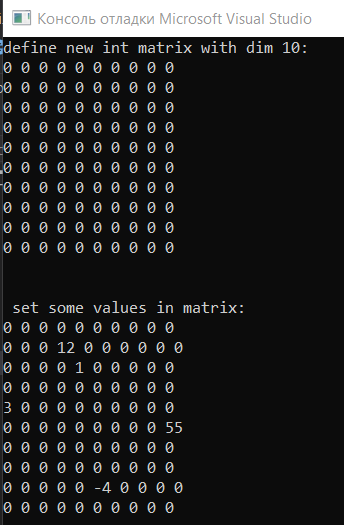
\includegraphics[width=300pt]{Test.png}
    \caption{перебор простой строки}
    \label{fig:my_label}
\end{figure}

\begin{figure}[H]
    \centering
    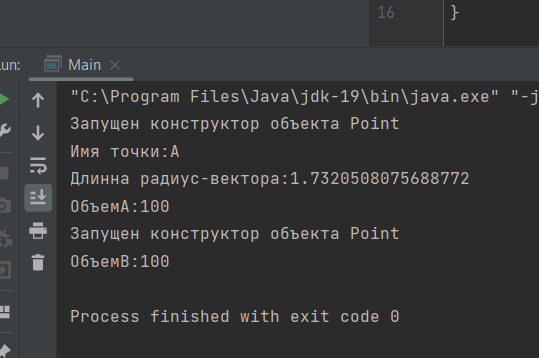
\includegraphics[width=300pt]{Test1.png}
    \caption{создание другой строки и её изменение}
    \label{fig:my_label}
\end{figure}

\begin{figure}[H]
    \centering
    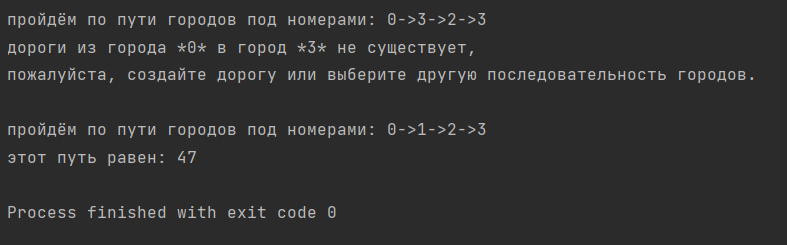
\includegraphics[width=400pt]{Test2.png}
    \caption{второй перебор}
    \label{fig:my_label}
\end{figure}


\end{document}